% A complete nonsingular fan in R^2 with five rays (a toric surface of Picard number 3).
\documentclass[border=2pt]{standalone}
\usepackage{tikz}
\usetikzlibrary{arrows.meta}
% Shared colours of the research figures (matplotlib tab10, as in the Berkovich skeleton figure).
\usepackage{amsmath}
\usetikzlibrary{calc}
\definecolor{figink}{HTML}{262626}
\definecolor{figred}{HTML}{D62728}
\definecolor{figblue}{HTML}{1F77B4}

\begin{document}
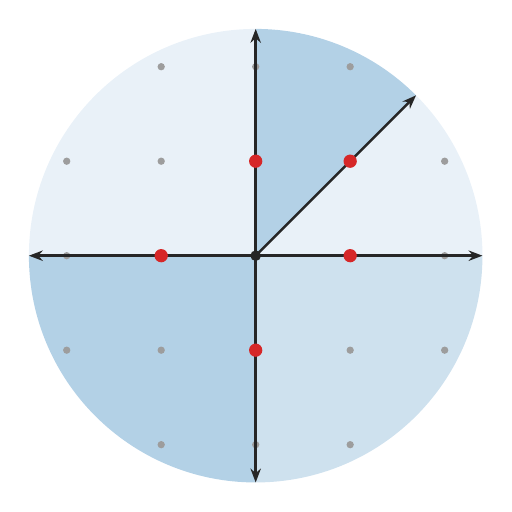
\begin{tikzpicture}[scale=1.2]
  \def\R{2.4}
  % the five 2-dimensional cones, as sectors of a disk
  \foreach \a/\b/\t in {0/45/10, 45/90/34, 90/180/10, 180/270/34, 270/360/22}
    \fill[figblue!\t] (0,0) -- (\a:\R) arc[start angle=\a, end angle=\b, radius=\R] -- cycle;
  % lattice points
  \begin{scope}
    \clip (0,0) circle (\R);
    \foreach \x in {-2,...,2} \foreach \y in {-2,...,2}
      \fill[figink!45] (\x,\y) circle (1.1pt);
  \end{scope}
  % rays, with their primitive generators
  \foreach \x/\y/\a in {1/0/0, 1/1/45, 0/1/90, -1/0/180, 0/-1/270} {
    \draw[figink, line width=0.9pt, -{Stealth[length=5pt]}] (0,0) -- (\a:\R);
    \fill[figred] (\x,\y) circle (2pt);
  }
  \fill[figink] (0,0) circle (1.6pt);
\end{tikzpicture}
\end{document}
